\chapter{Hydrogen Atom}
\section{Fine Structure}
\subsection{Lamb Shift}
An interesting feature of the fine structure formula is that it depends only on $j$ and not $l$, moreover in general two different values of $l$ share the same energy. For example, the $2S_{1/2} ()$ and $2P_{1/2} ()$ states should remain perfectly degenerate. However in 1947 Lamb and Retherford performed an experiment that displayed something to the contrary. The $S$ state is slightly higher in energy than the $p$ state. The explanation of this "Lamb" shift was later explained by Bethe, Feynman, Schwinger and Tomonaga (the founders of QED) as a corollary of the electromagnetic field itself being quantised.  Sharply in contrast to the hyperfine structure of Hydrogen, the Lamb shift is a completely novel i.e. non-classical (as the hyperfine structure is explained through Coulomb's law and the Biot-Savart Law) phenomena. It arises from a radiative correction in Quantum Electrodynamics to which classical theories are mute. In Feynman lingo, this arises from loop corrections as potrayed below.
\begin{figure}[h]
	\centering
	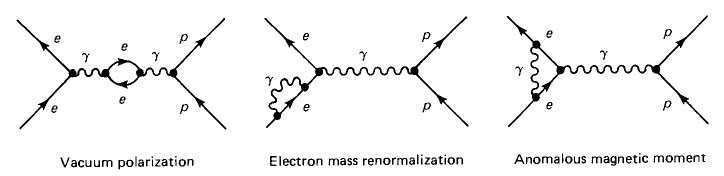
\includegraphics[width=0.6\linewidth, height=0.3\linewidth]{feyn-loop.png}
	\caption{Different kinds of radiative corrections}
\end{figure}
Naively,
\begin{enumerate}
\item the first diagram describes pair-production in the neighbhorhood of a nucleus, leading to a partial screening effect of the proton's charge;
\item the second diagram reflects the fact that the electromagnetic field has a non-zero ground state
\item the third diagram leads to a tiny modification of the electron's magnetic dipole moment (an addition of $a + \alpha/2\pi = 1.00116$)
\end{enumerate}
We shall not discuss the results in depth but rather consider two exemplary cases:\\
For $ l = 0$,
\begin{equation}
	\Delta E_{Lamb} = \alpha^{5}mc^{2}\frac{1}{4n^{3}}\left[k(n,0)\right]
\end{equation}
Where $k(n,0)$ is a numerical factor defined as:
$$k(n,0) = \begin{cases}
12.7, & \text{if } n = 1\\
13.2,              & \text{if } n \rightarrow \infty
\end{cases} $$
For $ l = 0$ and $j = l \pm \frac{1}{2}$,
\begin{equation}
\Delta E_{Lamb} = \alpha^{5}mc^{2}\frac{1}{4n^{3}}\left[ k(n,0) \pm \frac{1}{\pi (l + \frac{1}{2}) (l + \frac{1}{2})} \right]
\end{equation}
Here, $k(n,l)$ is a very small number $(< 0.05)$ which varies a little with it's arguments.\\
The Lamb shift is tiny except for the case $l=0$, for which it amounts to about $10 \% $ of the fine structure. However, since it depends on $l$, it lifts the degeneracy of the pairs of states with common $n$ and $j$ and in particular it splits $2 S_{1/2}$ and $2 P_{1/2}$.
\section{The Zeeman Effect}
When an atom is placed in a uniform magnetic field $B_{Ext.}$, the energy levels are shifted, this is known as the Zeeman effect. For the case of a single electron, the shift is:
\begin{equation}\label{zeeman_def}
H^{'}_{Z} = -(\mu_{l} + \mu_{s}).B_{Ext.}
\end{equation}
Where,
\begin{equation}
\mu_{s} = -\frac{e}{m_{e}}S
\end{equation}
is the magnetic dipole moment associated with electron spin, and
\begin{equation}
\mu_{l} = -\frac{e}{2m_{e}}L
\end{equation}
is the dipole moment associated with orbital motion. The gyromagnetic ratio in this case is simply classical i.e. $q/2m$, it is only for spin that we have an extra factor of 2. We now rewrite (\ref{zeeman_def}) as:
\begin{equation}
H^{'}_{Z} = \frac{e}{2m_{e}}(L + 2S).B_{Ext.}
\end{equation}
The nature of the Zeeman splitting depnds on the strength of the external field vs. the internal one that gives rise to spin-orbit/spin-spin coupling. This table provides a short review of the different cases:
\begin{center}
\begin{tabularx}{0.9\textwidth} { 
		| >{\centering\arraybackslash}X 
		| >{\centering\arraybackslash}X 
		| >{\centering\arraybackslash}X | }
	\hline
	\textbf{Case} & \textbf{Name} & \textbf{Comments} \\
	\hline
	$B_{Ext.} >> B_{Int.}$  & Strong-Field Zeeman Effect  & Zeeman effect dominates; fine structure becomes the perturbation  \\
	\hline
	$B_{Ext.} << B_{Int.}$  & Weak-Field Zeeman Effect  & Fine structure dominates; $H^{'}_{z}$ can be treated as a small perturbation   \\
	\hline
	$B_{Ext.} = B_{Int.}$  & Intermediate Zeeman Effect  & Both the fields are equal in strength thus we would need elements of degenerate peturbation theory and will need to diagonlize the necessary portion of the Hamiltonian "by hand" \\
	\hline
\end{tabularx}
\end{center}
In the next few sections we'll explore all of them in depth.
\subsection{Weak-Field Zeeman Effect}
Here the fine structure dominates, thus the conserved quantum numbers are $n$, $l$, $j$ and $m_{j}$, but not $m_{l}$ and $m_{s}$ due to the spin-orbit coupling L and S are not separately conserved. Generally speaking, in this problem we have a perturbation pile on top of a perturbation. Thus, the conserved quantum number are those appropriate to the dominant . In first order perturbation theory, the Zeeman correction to energy is,
\begin{equation}
E^{1}_{Z} = \expval{H^{'}_{Z}}{nlj m_{j}} = \frac{e}{2m}B_{Ext.} \expval{L + 2S}
\end{equation} 
Now to figure out $\expval{L + 2S}$, we know that $L + 2S = J + S$, this doesn't immediately tell us the expectation value of $S$ but we can figure it out as by understanding that $J = L + S$ is conserved and that the time average of $S$ is simply it's projection along $J$:
\begin{equation}
	S_{Ave} = \frac{(S.J)}{J}J
\end{equation}
But, $L = J - S$, so  $L^{2} = J^{2} + S^{2} - 2 J.S$, hence:
\begin{equation}
S.J = \frac{1}{2}(J^{2} + S^{2} - 2 J.S) = \frac{\hbar^{2}}{2}[j(j+1)+ s(s+1)-l(l+1)]
\end{equation}
from which it follows that,
\begin{equation}
	\expval{L + 2S} = \expval{\left(1 + \frac{S.J}{J^{2}}J\right)} = \left[1 + \frac{j(j+1)-l(l+1) + 3/4}{2j(j+1)}\right]\expval{J}
\end{equation}
The term in the square brackets is called the Lande g-factor, denoted by $g_{j}$. Now, if we choose $B_{z}$ to lie along $B_{Ext.}$, then:
\begin{equation}
	E^{1}_{Z} = \mu_{B} g_{j} B_{Ext.} m_{j}
\end{equation}
where,
$$\mu_{B} = \frac{e \hbar}{2m} = 5.788 \times 10^{-5} \ eVT^{-1}$$
is the so called Bohr magneton. The total energy is the sum of the fine-structure part and the Zeeman contribution, in the ground state i.e. $n = 1, l = 0, j = 1/2$ and therefore, $g_{J} = 2$, it splits into two levels:
\begin{equation}
	-13.6 \ eV(1 + \alpha^{2}/4) \pm \mu_{B} B_{Ext.}
\end{equation}
with different signs for different $m_{j}$'s this is plotted below.
\begin{figure}[h]
	\centering
	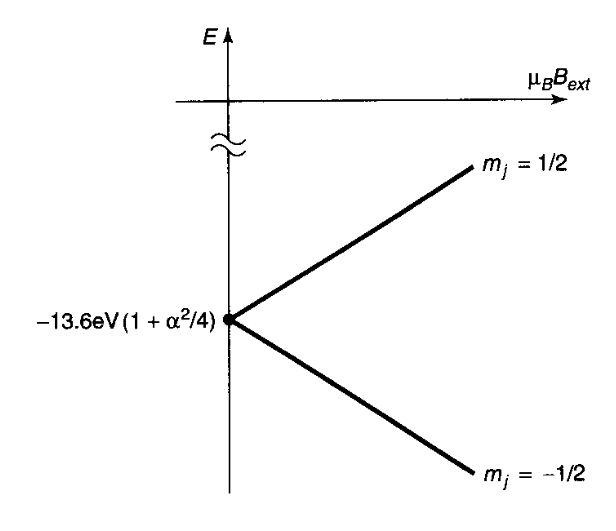
\includegraphics[width=0.6\linewidth, height=0.5\linewidth]{strong-split.png}
	\caption{Weak-field Zeeman splitting of the ground state of hydrogen; the upper line has a slope of $1$ and the lower line a slope of $-1$}
\end{figure}
\begin{figure}[h]
	\centering
	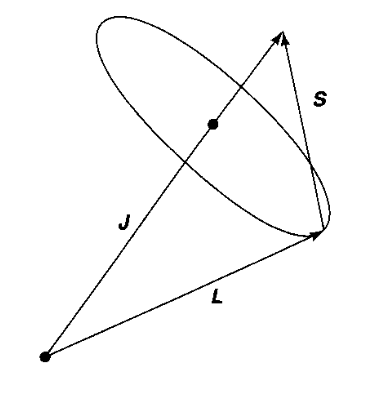
\includegraphics[width=0.6\linewidth, height=0.5\linewidth]{weak-split.png}
	\caption{In the presence of spin-orbit coupling, $L$ and $S$ are not separately conserved, they precess about the fixed total angular momentum $J$}
\end{figure}
\subsection{Strong-Field Zeeman Effect}
In this case, the Zeeman effect is often referred to as the "Paschen-Back" effect. The conserved quantum numbers are now but and because in the presence of an external torque, the total angular momentum is not conserved but the it's individual components are. The Zeeman Hamiltonian is,
\begin{equation}
H^{'}_{Z} =  \frac{e}{2m} B_{Ext.} (L_{z} + 2 S_{z})
\end{equation}
and the unperturbed energies are:
\begin{equation}
	E_{nm_{l}m_{s}} = -\frac{13.6 \ eV}{n^{2}} + \mu_{B}B_{Ext.}(m_{l} + 2 m_{s})
\end{equation}
This would be our result if we ignore the fine structure completely. However, we need to take that into account as well. In first-order perturbation theory, the fine structure correction to these levels is:
\begin{equation}
E^{1}_{fs} = \expval{H^{'}_{r} + H^{'}_{so}}{n \ l \ m_{l} \ m_{s}}
\end{equation}
The relativistic contribution is the same as before for the spin-orbit term, we need
\begin{equation}
\expval{S.L} = \expval{S_{x}}\expval{L_{x}} + \expval{S_{y}}\expval{L_{y}} + \expval{S_{z}}\expval{L_{z}} = \hbar^{2}m_{l}m_{s}
\end{equation}
Here $\expval{S_{x}} = \expval{S_{y}} = \expval{L_{x}} = \expval{L_{y}} = 0$ for the eigenstates of $S_{z}$ and $L_{z}$. Putting it all together:
\begin{equation}
E^{1}_{fs} = \frac{13.6 \ eV}{n^{3}}\alpha^{2} \left(\frac{3}{4n} - \left[ \frac{l(l+1)-m_{l}m_{s}}{l(l+1/2)(l+1)}\right]\right)
\end{equation}
Th term in the square brackets is indeterminate for $l=0$, it's correct value in this case is 1. The total energy here is the sum of the Zeeman part and the fine structure contribution.
\subsection{Intermediate Zeeman Effect}
In this case, we must treat both the effects as perturbations to the Bohr Hamiltonian,
\begin{equation}
H^{'} = H^{'}_{Z} + H^{'}_{fs}
\end{equation}
In section we'll discuss the case $n = 2$, and use it as the basis for degerate perturbation theory. The states here are characterized by $l$, $j$ and $m_{j}$. We could use $l$,$m_{l}$,$m_{s}$ states but this makes the matrix elements of $H^{'}_{Z}$ easier to deal with but that of $H^{'}_{fs}$ difficult. Using the Clebsch-Gordan coefficients to express $\ket{j m_{j}}$ as a linear combination of $\ket{l m_{l}} \ket{s m_{s}}$ we have:
$$l = 0 = \begin{cases}
\psi_{1} & \ket{\frac{1}{2} \frac{1}{2}} = \ket{0 \ 0}\ket{\frac{1}{2}\frac{1}{2}}\\
\psi_{2} & \ket{\frac{1}{2} \frac{-1}{2}} = \ket{0 \ 0}\ket{\frac{1}{2}\frac{-1}{2}}
\end{cases} $$
$$l = 1 = \begin{cases}
\psi_{3} & \ket{\frac{3}{2} \frac{3}{2}} = \ket{1 \ 1}\ket{\frac{1}{2}\frac{1}{2}}\\
\psi_{4} & \ket{\frac{3}{2} \frac{-3}{2}} = \ket{1 \ -1}\ket{\frac{1}{2}\frac{-1}{2}}\\
\psi_{5} & \ket{\frac{3}{2} \frac{1}{2}} = \sqrt{2/3}\ket{1 \ 0}\ket{\frac{1}{2}\frac{1}{2}} + \sqrt{1/3}\ket{1 \ 1}\ket{\frac{1}{2}\frac{-1}{2}}\\
\psi_{6} & \ket{\frac{1}{2} \frac{1}{2}} = -\sqrt{1/3}\ket{1 \ 0}\ket{\frac{1}{2}\frac{1}{2}} + \sqrt{2/3}\ket{1 \ 1}\ket{\frac{1}{2}\frac{-1}{2}}\\
\psi_{7} & \ket{\frac{3}{2} \frac{-1}{2}} = \sqrt{1/3}\ket{1 \ -1}\ket{\frac{1}{2}\frac{1}{2}} + \sqrt{2/3}\ket{1 \ 0}\ket{\frac{1}{2}\frac{-1}{2}}\\
\psi_{8} & \ket{\frac{1}{2} \frac{-1}{2}} = -\sqrt{2/3}\ket{1 \ -1}\ket{\frac{1}{2}\frac{1}{2}} + \sqrt{1/3}\ket{1 \ 0}\ket{\frac{1}{2}\frac{-1}{2}}\\
\end{cases} $$
In this basis the matrix the non-zero elements of $H^{'}_{fs}$ are all on the diagonal and are given by the Bohr model. $H^{'}_{z}$ has four off diagonal elements. The complete matrix, W as we will see is more complicated but its eigenvalues are the same since they are independent of the chosen basis.
\begin{equation}
\begin{pmatrix}
5 \gamma - \beta & 0 & 0 & 0 & 0 & 0 & 0 & 0 \\
0 & 5 \gamma + \beta & 0 & 0 & 0 & 0 & 0 & 0\\
0 & 0 & \gamma - 2 \beta & 0 & 0 & 0 & 0 & 0\\
0 & 0 & 0 & \gamma + 2 \beta & 0 & 0 & 0 & 0\\
0 & 0 & 0 & 0 & \gamma - \frac{2}{3} \beta & \frac{\sqrt{2}}{3} \beta & 0 & 0\\
0 & 0 & 0 & 0 & \frac{\sqrt{2}}{3} \beta & 5 \gamma - \frac{1}{3} \beta & 0 & 0\\
0 & 0 & 0 & 0 & 0 & 0 & \gamma + \frac{2}{3} \beta & \frac{\sqrt{2}}{3} \beta\\
0 & 0 & 0 & 0 & 0 & 0 & \frac{\sqrt{2}}{3} \beta & 5 \gamma + \frac{1}{3} \beta
\end{pmatrix}
\end{equation}
Where,
$$\gamma = {(\alpha / 8)}^{2}13.6 \ eV$$
and,
$$\beta = \mu_{B}B_{Ext.}$$
The first four eigenvalues are already displayed along the diagonal. We only need to find the eigenvalues of the two  $2 \times 2$ blocks. The characteristic equation for the first one is given as:
\begin{equation}
	\lambda^{2} - \lambda(6\gamma - \beta) + \left(5 \gamma^{2} - \frac{11}{3} \gamma \beta\right) = 0
\end{equation} 
and the quadratic formula gives the eigenvalues:
\begin{equation}
\lambda_{\pm} = 3 \gamma - (\beta /2) \pm \sqrt{4 \gamma^{2} + (2/3) \gamma \beta + (\beta^{2}/4)} 
\end{equation}
The eigenvalues of the second block are the same but with the sign of $\beta$ reversed. The eight energy levels are listed in the table and are plotted against in the figure (). In the zero field limit they reduce to the fine structure values. For the other cases, the splitting is seen clearly.
\begin{figure}[h]
	\centering
	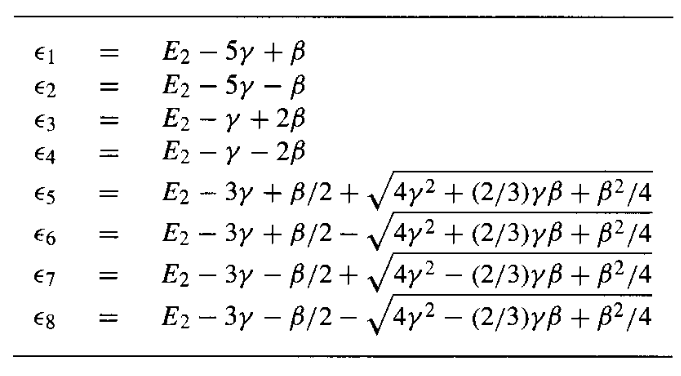
\includegraphics[width=0.6\linewidth, height=0.3\linewidth]{zee-table.png}
	\caption{Energy levels for the $n=2$ states of hydrogen, with fine structure and Zeeman splitting}
\end{figure}
\begin{figure}[h]
	\centering
	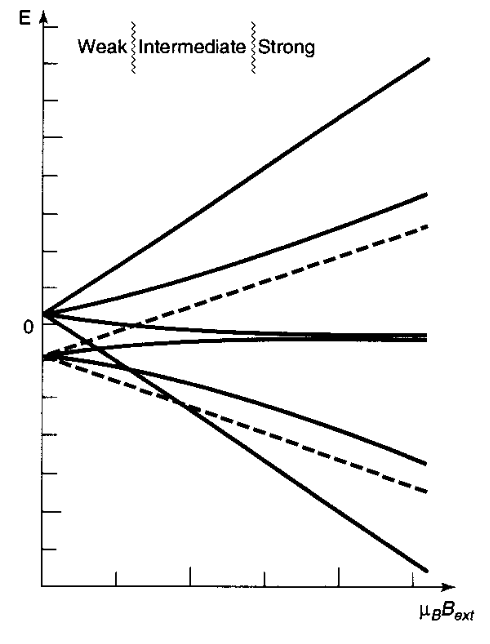
\includegraphics[width=0.6\linewidth, height=0.6\linewidth]{intermediate-split.png}
	\caption{Zeeman splitting of the $n = 2$ states of hydrogen, in the weak, intermediate and strong field regimes}
\end{figure}
\section{Hyperfine Splitting in Hydrogen}
The proton also has a magnetic dipole moment, however this is much smaller than that of the electron due to the mass of the proton. It is given by,
\begin{equation}
	\mu_{p} = \frac{g_{p} e}{2 m_{p}}S_{p}
\end{equation}
And the magnetic dipole moment of the electron,
\begin{equation}
\mu_{e} = -\frac{e}{m_{e}}S_{e}
\end{equation}
Classically speaking, the dipole $\mu$ sets up a magnetic field:
\begin{equation}
	B = \frac{\mu_{0}}{4 \pi r^{3}}[3(\mu . \hat{r})\hat{r} - \mu] + \frac{2 \mu_{0}}{3} \mu \delta^{3}(r)
\end{equation}
So the Hamiltonian of the electron, in the magnetic field due to the proton's magnetics dipole moment, is
\begin{equation}
	H^{'}_{hf} = \frac{\mu_{0} g_{p} e^{2}}{8 \pi m_{p} m_{e}}\frac{[3(S_{p}. \hat{r})(S_{e}. \hat{r}) - S_{p}.S_{e}]}{r^{3}} + \frac{\mu_{0} g_{p} e^{2}}{3 m_{p} m_{e}}S_{p}.S_{e} \delta^{3}(r)
\end{equation}
According to perturbation theory, the first-order correcction to the energy is the expectation value of the perturbing Hamiltonian:
\begin{equation}
	E^{1}_{hf} = \frac{\mu_{0} g_{p} e^{2}}{8 \pi m_{p} m_{e}} \expval{\frac{3(S_{p}.\hat{r})(S_{e}.\hat{r}) - S_{p}.S_{e}}{r^{3}}} + \frac{\mu_{0} g_{p} e^{2}}{3 m_{p} m_{e}}\expval{S_{p}.S_{e}}\abs{\psi(0)}^{2}
\end{equation}
In the groud state or any other state at which $l = 0$, the wavefunction is spherically symmetrical, and the first expectation value vanishes. Meanwhile, from the Schrodinger equation in three dimensions, we find that $\abs{\psi(0)}^{2} = 1/(\pi a^{3})$, thus,
\begin{equation}
E^{1}_{hf} = \frac{\mu_{0} g_{p} e^{2}}{3 \pi m_{p}m_{e} a^{3}}\expval{S_{p}.S_{e}}
\end{equation}
in the groud state. This is called Spin-Spin coupling because it involves the dot product of two spins in contrast with spin-orbit coupling which involves $S.L$. In the presence of spin-spin coupling, the individual spin angular momenta are no longer conserved. However the eigenvectors of the total spin is conserved:
\begin{equation}
S = S_{e} + S_{p}
\end{equation}
We square this out to get,
\begin{equation}
	S_{p}. S_{e} = \frac{1}{2}(S^{2} - S^{2}_{e} - S^{2}_{p})
\end{equation}
But the electron and proton both have spin $1/2$, so $S^{2}_{e} = S^{2}_{p} = (3/4) \hbar^{2}$. In the triplet i.e. parallel spin state, the total spin is $1$, and hence $S^{2} = 2 \hbar^{2}$. In the singlet state the total spin is $0$, and  $S^{2} = 0$. Thus,
\begin{equation}
E^{1}_{hf} = \frac{4 g_{p} \hbar^{4}}{3 m_{p} m^{2}_{e}c^{2}\alpha^{4}} \begin{cases}
+1/4, & \text{ (triplet)};\\
-3/4, & \text{ (singlet)}
\end{cases}
\end{equation}
The Spin-Spin coupling breaks the spin degeneracy of the groud state, lifting the triplet and depressing the singlet, leading to an energy gap. The energy gap is given by:
\begin{equation}
	\Delta E = \frac{4 g_{p} \hbar^{4}}{3 m_{p} m^{2}_{e}c^{2}\alpha^{4}} = 5.88 \times 10^{-6} \ eV
\end{equation}
\begin{figure}[h]
	\centering
	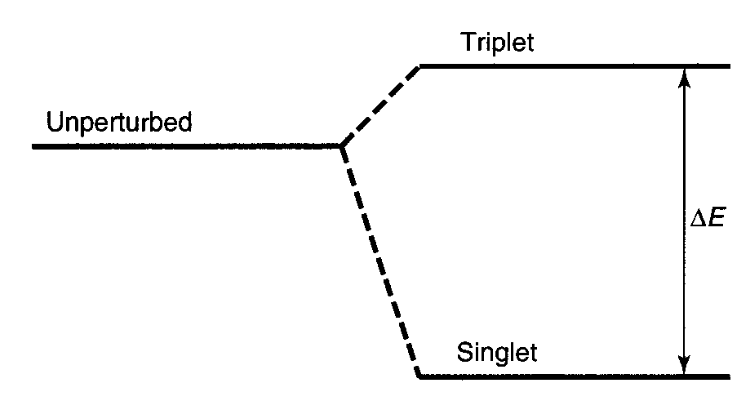
\includegraphics[width=0.6\linewidth, height=0.3\linewidth]{hyp-split.png}
	\caption{Hyperfine splitting in the ground state of Hydrogen}
\end{figure}
The frequency of the photon emitted when the triplet transitions to a singlet state is:
\begin{equation}
	\nu = \frac{\Delta E}{h} = 1420 \text{ MHz}
\end{equation}
The corresponding wavelength is $21 $ cm which falls in the microwave region. It permeates the universe and is a very important part of Astrophysics.
